\chapter{Estrellas}

Las \textbf{estrellas} son de los objetos más fundamentales e importantes en el
estudio de los astros. \citetbookchapter{anIntroStellarAstro}{1} define una
estrella como \quotes{un objeto celeste en el cual existe, o alguna vez existió
(en el caso de una estrella muerta) fusión de hidrógeno sostenido en su núcleo.}
El núcleo de cada estrella activa alcanza temperaturas en el orden de decenas de
millones de Kelvin, lo cual permite generar nuevos elementos más pesados mediante el
proceso de fusión nuclear. El mecanismo principal para la generación de energía
es la fusión de hidrógeno a helio: $\ce{4 ^1H} \rightarrow \ce{^4He} + E$ .
Dentro de todas las estrellas existe un balance de fuerzas que mantiene la forma
esférica de la estrella; esto se le conoce como el \textit{equilibrio
hidrostático}, en el cual la presión interna de la estrella tiene una
contra-fuerza equivalente del peso de su mismo gas. Este balance es modelado a
escalas menores a las de las propiedades macroscópicas de la estrella
(\citetbookchapter{anIntroTheoryStellarStructureEvolution}{2}), en la cual la
estrella está en un estado de \textit{equilibrio termodinámico local}. 

Una estrella está caracterizada por sus propiedades físicas, como su masa,
composición química, radio, y temperatura. A continuación se plantea una base
para describir la estructura de una estrella al igual que su evolución,
empezando con la formación de una \textit{protoestrella}, la cual con el paso del
tiempo se transforma en una estrella.

\section{Formación}

El \textbf{medio interestelar} (ISM por sus siglas en inglés) es la región de
espacio que existe entre el Sol y el resto de las estrellas dentro de nuestra
Galaxia. Está compuesto de todo el polvo, gas, y partículas libres como los
rayos cósmicos que atraviesan el espacio. La distribución de este material no es
uniforme a cortas escalas de distancias astronómicas, por lo cual se observan
acumulaciones de gas y polvo que se les conoce como \textbf{nubes moleculares}.
Estas nubes se encuentran a temperaturas extremadamente frías, hasta los
10-20 K en su estado de equilibrio. Sin embargo, la nube puede llegar a ser
perturbada de este estado, lo cual causa una distribución de masa y un campo
gravitacional no uniforme, dando forma a cúmulos densos de material.

% TODO: probably add symbols table in thesis for M_\odot (and probably others to
% be used in rest of doc)

Dado suficiente tiempo una nube molecular va colapsando bajo su propio peso,
donde la presión en la nube provoca que el material se acumule en un solo punto en
el espacio. Mientras más aumente la presión el gas se calienta; este proceso
sigue hasta llegar a un equilibrio entre la presión interna del gas y la fuerza
compresiva de gravedad, en donde la nube deja de contraerse. Dependiendo de la
temperatura a la que alcanza el núcleo determina si se convierte en una estrella
capaz de mantener una reacción continua de fusión nuclear. La masa mínima para
que una nube molecular colapse a una estrella es de $0.08 \ \mathrm{M}_{\odot}$
(\citetbookchapter{anIntroStellarAstro}{2}). De no cumplir con esta condición, el
cúmulo de gas y polvo no logrará mantener la cadena de reacciones termonucleares
en su núcleo, resultando en una \textit{enana café}, un objeto inerte resultado
del proceso fallido de formación estelar.

Una vez que el material de la nube se estabilice\textemdash una vez que el
objeto empiece a producir energía de orden de magnitud estelar\textemdash nace
una \textbf{protoestrella}. Estos objetos extensos (aproximadamente $500 \
\mathrm{R}_{\odot}$ para una protoestrella de $1 \ \mathrm{M}_{\odot}$
(\citetbookchapter{astronomyPhysicalPerspective}{15})) se mantienen a una baja
temperatura durante esta etapa de su vida, alrededor de 2500 K en su superficie.
Sin embargo, debido a la alta densidad, la nube no es completamente
transparente, por lo cual solo la superficie es capaz de liberar energía por
medio de radiación infrarroja; la energía producida en su interior primero debe
de viajar a la superficie por medio de convección. Conforme va evolucionando la
nube se sigue comprimiendo hasta llegar a un punto en el cual puede mantener
reacciones termonucleares continuas en su núcleo, llegando al punto de ser una
estrella en \textbf{secuencia principal}. La \reffigure{protostarEvolutionFig}
muestra la evolución de una protoestrella a una estrella secuencia principal con
respecto a su masa.

\begin{figure}[!ht]
	\centering
	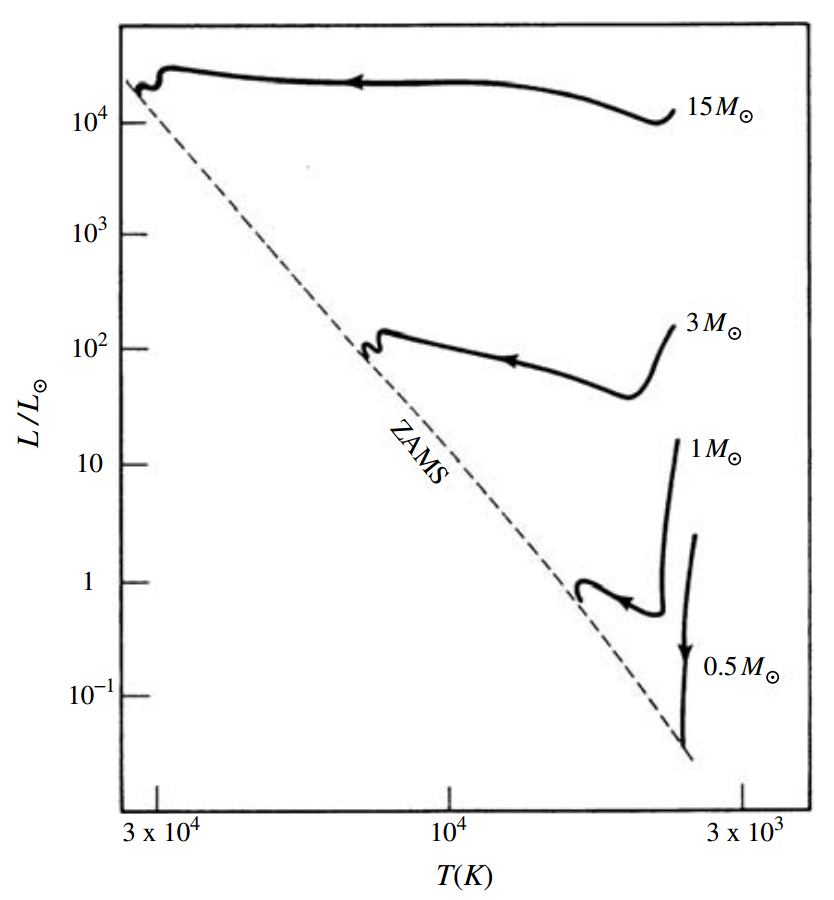
\includegraphics[scale=0.27]{Introduccion/Figures/EvolucionZAMSFormacionEstelar_Kutner.png}
	\caption{Diagrama de la evolución de una protoestrella hasta llegar a
	\textit{ZAMS} (\textit{Zero Age Main Sequence}), la edad a la que se
	convierte en una estrella de secuencia principal. Se muestran varios caminos
	evolutivos de una protoestrella en función de su masa, el cual es el
	parámetro de mayor importancia en su evolución y estado final. Figura
	obtenida de \citetbookchapter{astronomyPhysicalPerspective}{15}.}
	\label{protostarEvolutionFig}
\end{figure}

\section{Secuencia Principal}

Una vez que una estrella llegue su etapa de secuencia principal el sistema se
vuelve estable a largas escalas temporales. En este estado la estrella deja de
comprimirse, ya que el colapso gravitacional es contrarrestado por la presión
del gas caliente en su interior y la presión ejercida por la radiación producida
en su núcleo. A continuación se definen dos conceptos importantes en la física
estelar: el \textbf{equilibrio hidrostático} y el \textbf{equilibrio
termodinámico local}.

\subsection{Equilibrio Hidrostático}

Podemos simplificar el modelo de una estrella al introducir la simetría
esférica, en el cual las propiedades del gas que forma la estrella dependen
unicamente de la distancia del núcleo. Para esto definimos la presión $P(r)$,
densidad $\rho (r)$, temperatura $T(r)$, y aceleración gravitacional $g(r)$ como
funciones con respecto a la distancia $r$ del centro. En base a estos
fundamentos se puede deducir la estratificación de una estrella, formando varias
capas de material con propiedades uniformes a lo largo de cada estrato. Dado que
cada elemento dentro de la estrella está sujeto a un equilibrio de fuerzas descrita 
por la ecuación $P(r) \mathrm{d}A - [P(r) + \mathrm{d}P] \mathrm{d}A - [\rho(r) 
\mathrm{d}A \mathrm{d}r] g(r) = 0$, la cual se ve en la
\reffigure{figuraEquilibrioHidrostatico}, al simplificar esta ecuación e
introduciendo un término para la presión radiativa\textemdash debido a la
transferencia de momento de los fotones generados en el núcleo estelar al
material circundante\textemdash se obtiene la
\refequation{ecuacionEquilibrioHistrostatico}. 

\begin{eqfloat}[!ht]
	\centering
	\begin{equation}
		\frac{\textrm{d}P(r)}{\textrm{d}r} = -\rho(r) [g(r) - g_{rad}(r)]
	\end{equation}
	\caption{Ecuación del equilibrio hidrostático para una estrella, tomando en
	cuenta los efectos de la presión radiativa saliente $g_{rad}(r)$.
	\citetbookchapter{anIntroStellarAstro}{2}}
	\label{ecuacionEquilibrioHistrostatico}
\end{eqfloat}

\begin{figure}[!ht]
	\centering
	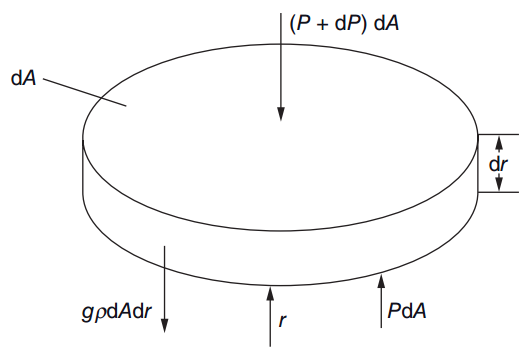
\includegraphics[scale=0.5]{Introduccion/Figures/EquilibrioHidrostatico_LeBlanc.png}
	\caption{Diagrama de fuerzas actuando sobre cada elemento dentro de la estrella con 
	área $\mathrm{d}A$ de material de una estrella. Los efectos debido a elementos
	adyacentes son nulos, debido a que la presión en cada lados es constante,
	resultando en un gradiente de presión radial. Figura obtenida de
	\citetbookchapter{anIntroStellarAstro}{2}.}
	\label{figuraEquilibrioHidrostatico}
\end{figure}

\subsection{Equilibrio Termodinámico Local}

Una estrella como resultado de su mecanismo de transporte de energía no está en
un estado de equilibrio térmico. El núcleo, en donde se produce la gran mayoría
de energía en una estrella, está a ordenes de magnitud más caliente que la
fotósfera. Este transporte de energía ocurre principalmente por medio de
\textit{radiación} y \textit{convección}; la conducción no juega un papel
significativo ya que el camino libre medio de las partículas de gas es grande. 
Para que una estrella se mantenga estable durante los miles de
millones de años de su vida debe de estar en un tipo de equilibrio, donde cada
capa mantiene una composición estable a largas escalas de tiempo,
lo cual implica que el flujo de energía que ingresa a cada capa es igual a la
cantidad de energía que libera a la siguiente capa. Esto lleva a cabo otra
simplificación en el modelo estelar: una estrella la podemos considerar como un
sistema en \textbf{equilibrio termodinámico local}.

Para declarar que un sistema está en equilibrio termodinámico local debemos
considerar el \textbf{camino libre medio} de una partícula en el interior
estelar. Considerando la distancia recorrida por un fotón antes de ser absorbido
o esparcido por otra partícula obtenemos esta medición, la cual dicta la escala
de espacio del transporte de energía comparado a la escala espacial de la
estrella. En el caso de que el camino libre medio sea significativamente menor
que las dimensiones espaciales de la estrella su volumen se puede dividir en
celdas discretas de tamaño despreciable, en las cuales cada una de las celdas
está en equilibrio termodinámico dentro de si mismas
(\citetbookchapter{anIntroTheoryStellarStructureEvolution}{2}). Por lo tanto, la
estructura de la estrella se puede determinar siempre y cuando se sepa la masa
de la estrella, y la densidad, temperatura, y composición química de cada punto
en su interior.

\section{Atmósfera Estelar}

La gran mayoría de la radiación que recibimos de las estrellas\textemdash tanto
de nuestro Sol como de sistemas estelares ajenos\textemdash proviene de su
\textbf{fotósfera}, la capa exterior sometida a la influencia gravitacional del
astro. Debido al transporte de energía en las capas interiores la fotósfera
se encuentra a una temperatura a ordenes de magnitud menor que la temperatura en
el núcleo; la intensidad monocromática de la estrella depende de esta
temperatura, por lo cual la \textbf{distribución de energía espectral}
(\textbf{SED} por sus siglas en inglés) varía de la misma forma.

Un \textbf{cuerpo negro} es aquel objeto que se encuentra en un estado de
equilibrio termodinámico con su ambiente, absorbiendo energía (en el caso de una
estrella esta sería por medio de radiación) a la misma tasa que la emite
(\citetbookchapter{astronomyPhysicalPerspective}{2}). El espectro de un cuerpo
negro está descrito por la función de Planck
(\refequation{blackbodyPlanckEquation}), de la cual obtenemos la intensidad para
cada longitud de onda dada la temperatura del cuerpo negro. La distribución
espectral de energía se puede ver en la \reffigure{figuraCuerpoNegroEspectro}.
Esta aproximación, a pesar de omitir una parte apreciable de la composición de
una estrella, es suficientemente adecuada para ciertos estudios donde no es
necesario implementar un modelo complejo.

\begin{eqfloat}
	\centering
	\begin{equation}
		B_\lambda (T) = \frac{2hc^2 / \lambda^5}{\mathrm{e}^{hc/\lambda kT} - 1}
	\end{equation}
	\caption{Función de Planck describiendo la intensidad emitida por un cuerpo
	negro con temperatura $T$ para una longitud de onda $\lambda$. $h$ es la
	constante de Planck, $k$ la constante de Boltzmann, y $c$ la velocidad de la
	luz en un vacío.}
	\label{blackbodyPlanckEquation}
\end{eqfloat}

\begin{figure}[!ht]
	\centering
	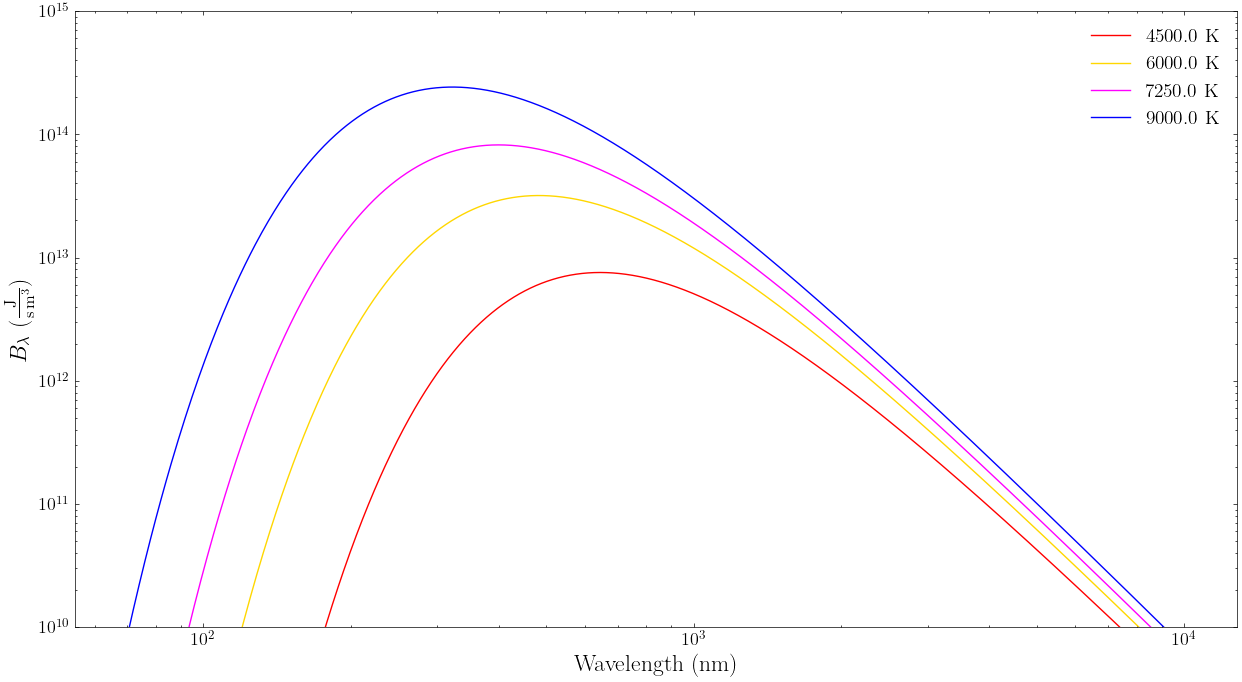
\includegraphics[scale=0.4]{Introduccion/Figures/Figura Cuerpo Negro Espectro.png}
	\caption{Intensidad de un cuerpo negro con temperatura efectiva especificada.}
	\label{figuraCuerpoNegroEspectro}
\end{figure}

Sin embargo, en la práctica la composición química de una estrella (conocido
como su \textbf{metalicidad}) llega a tener un efecto notable en su distribución
espectral de energía medida. Esto se debe a la absorción, dispersión, y emisión
de fotones por parte de las partículas en la atmósfera estelar, incluyendo
electrones y iones libres, átomos, y moléculas esparcidas dentro de este
volumen. Cada partícula interacciona con fotones de manera distinta, incluyendo
la tasa de interacciones con respecto a la frecuencia de la radiación incidente.
Existen varios códigos diseñados para modelar este comportamiento, llamados
\textbf{model atmospheres} en inglés. Estos códigos reciben de entrada los
parámetros conocidos de la estrella que se quiere modelar, su temperatura
efectiva, aceleración gravitacional superficial, y metalicidad (en unidades
solares), dando como resultado el espectro de la estrella.

\subsection{Atmósfera de Kurucz}

Entre los códigos de modelos de atmósferas estelares más utilizados está el de
\code{ATLAS} escrito por Robert L. Kurucz. A continuación se especifican las
suposiciones empleadas en el código de \code{ATLAS} descritas por
\citetbooksection{phoebeScientificReference}{4.2}; para una discusión completa
del programa es necesario hacer referencia a \citeyearparen{kurucz_atlas_1970}.

Este modelo parte de las condiciones del \textit{equilibrio hidrostático} y el
\textit{equilibrio termodinámico local} para una estrella, lo cual simplifica el
problema a un trato unidimensional; las propiedades físicas de la atmósfera
dependen únicamente de su distancia al núcleo. El grosor de cada capa es ordenes
de magnitud menor que la superficie que abarca la fotósfera estelar, lo cual
permite modelar dicha capa usando varios segmentos discretos que se aproximan a
\textit{planos paralelos}. La simetría esférica produce \textit{capas
homogéneas}, cuyas propiedades físicas como su composición química es uniforme
en cada capa, solo variando con su profundidad. Esto también permite ignorar
estructuras finas en la superficie de la estrella como la granulación y las
manchas solares (en ciertos ajustes de modelos estas manchas aún son requeridas
para un ajuste adecuado a los datos observacionales dados como se presenta en el
\refthesischapter{metodologia:modelocomputacional}). 

\begin{figure}[!ht]
	\centering
	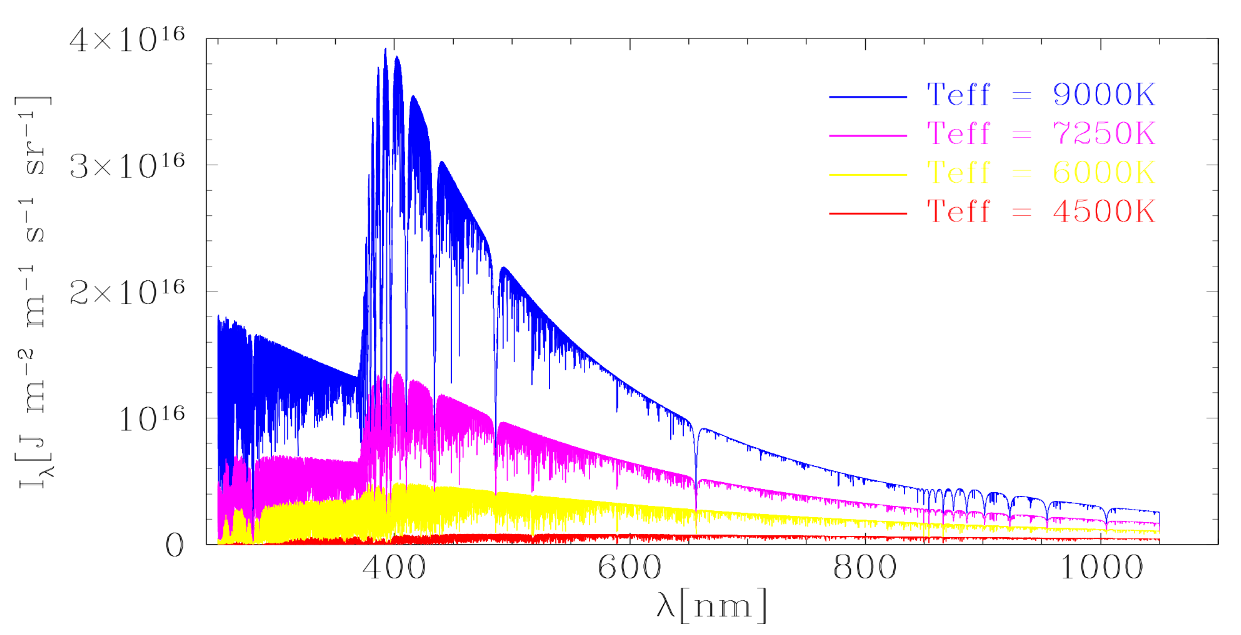
\includegraphics[scale=0.29]{Introduccion/Figures/Figura Kurucz_PHOEBE Reference.png}
	\caption{Espectros sintéticos de las tablas de Kurucz para estrellas de
	varias temperaturas. El resto de los parámetros físicos utilizados se
	mantuvieron fijos para los cuatro modelos: $\log{g/g_0} = 4.0$ y [M/H] =
	0.0. Figura obtenida de \citetbooksection{phoebeScientificReference}{4.2}.}
	\label{figuraKuruczEspectro}
\end{figure}

La \reffigure{figuraKuruczEspectro} muestra el espectro sintético generado por
el código \code{ATLAS} dado diferentes parámetros físicos. Estas aproximaciones
son ideales para estudiar estrellas aisladas, las cuales son mayormente
esféricas en forma. Sin embargo, este modelo tiene limitaciones significantes
para estrellas deformes, como los sistemas binarios cercanos donde las fuerzas
de marea causan una partida notable de su forma esférica. A pesar de no ser un
modelo perfecto, en la mayoría de los casos es más adecuado utilizar un código
como \code{ATLAS} que modelar una estrella como un simple cuerpo negro.

\section{Evolución}

Con el transcurso del tiempo cada estrella estará sujeta a ciertos cambios en su
estructura. Esto se debe a que podemos considerar a una estrella cómo un objeto
aislado en el espacio, lo cual significa que no tendrá algún ingreso de material
significativo para reemplazar el combustible \quotes{quemado} en las reacciones
termonucleares. A lo largo del tiempo la composición física y química de la
estrella deberán cambiar para mantener el equilibrio termodinámico.

El combustible primario de una estrella viene siendo el hidrógeno atómico, el
cual se fusiona con otros átomos (protones individuales) libres, resultando en
la producción de grandes cantidades de energía en forma de radiación y moléculas
de helio como producto. El helio no es inmediatamente útil para la estrella cómo
combustible, ya que requiere temperaturas más altas de las que se encuentran
durante esta fase evolutiva. Todas las estrellas conocidas pasan por esta etapa
de evolución estelar; mientras que una estrella dependa principalmente del
hidrógeno para brillar se dice que está en su etapa de \textit{secuencia
principal}. 

\begin{figure}[!ht]
	\centering
	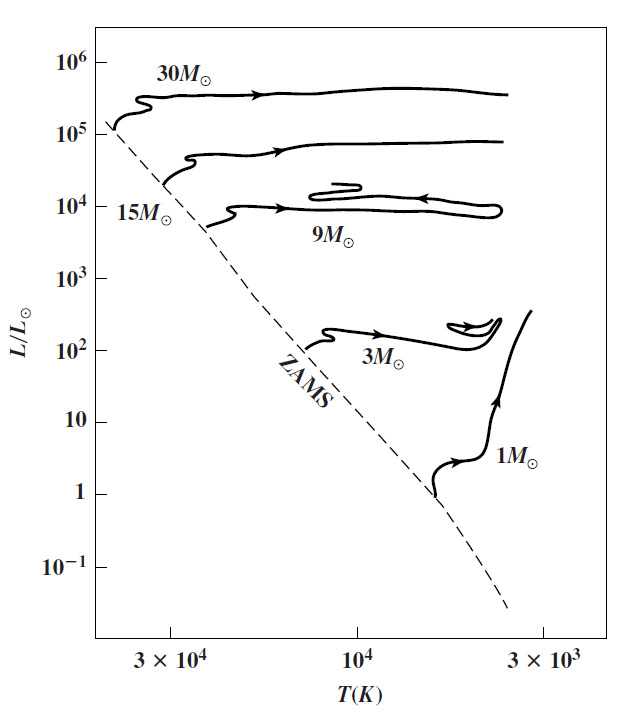
\includegraphics[scale=0.43]{Introduccion/Figures/Figura Evolucion_MS_Astronomy_Physical_Perspective.png}
	\caption{Evolución de estrellas de la secuencia principal basado en su masa
	inicial en el diagrama HR. La línea punteada representa la posición de la
	estrella en el primer momento que se integra a la secuencia principal. Al
	consumir el hidrógeno en su núcleo por las reacciones nucleares que ocurren
	en esta misma región se comienza a desatar el equilibrio delicado que
	mantiene la forma de la estrella. Esta deformación provoca una oscilación en
	su tamaño, causado por las fluctuaciones del balance entre la presión
	radiativa generada por las reacciones nucleares en el núcleo contra la
	presión gravitacional. Diagrama obtenido de
	\citetbookchapter{astronomyPhysicalPerspective}{2}}
	\label{evolucionMSEstrella}
\end{figure}